\chapter{Implementation}

\pagebreak

\section{Hardware Applications}

Since this project and study was purely an algorithmic implementation and product engineering showcase, the hardware required is extremely minimal and found in abundance with most consumers. All the project requires is a Windows/Mac/Linux PC that has minimum system hardware requirements to build the source, and an Android/iOS device with Google Assistant or Facebook Messenger installed to be able to test and run the application.

\section{Software Applications}

\begin{itemize}
    \item Operating System: Mac, Linux, Windows 8/10
    \item Programming Languages: Python, Node.js
    \item Chatbot Framework: DialogFlow
    \item Deep Learning Framework: Tensorflow
    \item Editors: Visual Studio Code, Jupyter Notebook
    \item Server: Heroku
\end{itemize}

\pagebreak

\section{Procedure}

This section extensively talks about the artificial intelligence involved in our project.

\subsection{Project File Structure}

Organizing files on your computer is just like organizing anything else. Say you want to organize your clothes. You might sort each type of clothes into separate stacks. Then you might pair the socks or group all the shirts by color. Or, you could throw everything into one drawer and hope you can find the right pair of socks when you need it. And that's how we typically treat our files: we save files randomly to our Desktop and Documents folders, then waste time searching for files every day.

\begin{figure}[H]
    \centering
    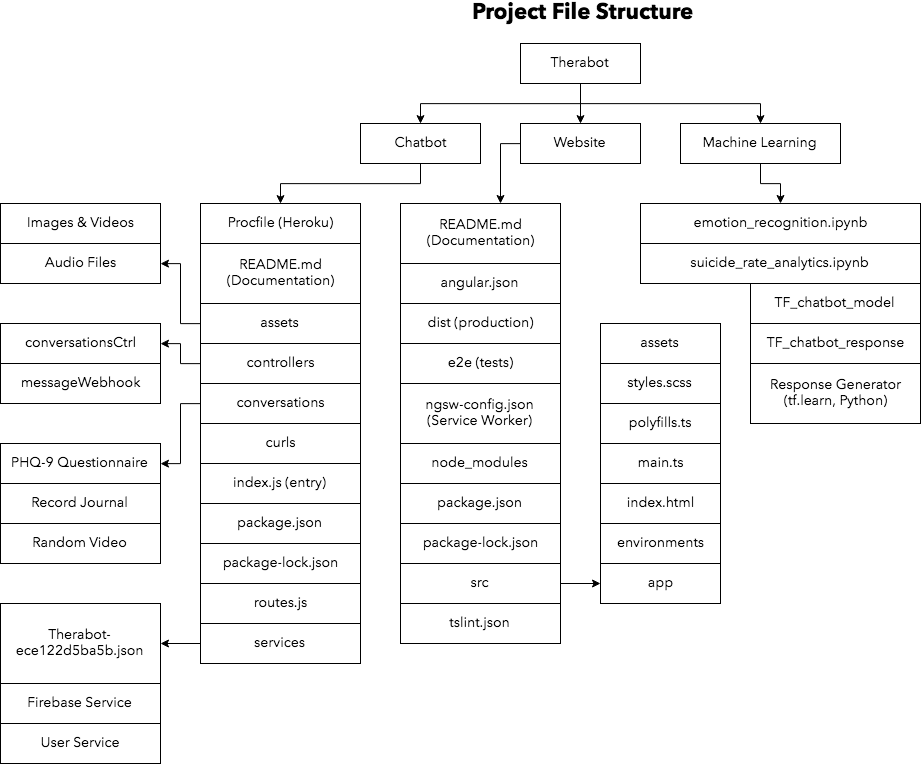
\includegraphics[width=12cm]{images/project-file-structure.png}
    \caption{Project File Structure}
\end{figure}

Folder structures can help, just like drawers and dividers can keep your clothes organized. A folder structure is the way folders are organized on your computer. As folders are added over time, you can either keep them at the same level—like Folders 1, 2, and 3 in the chart below—or nest them within each other for a hierarchy—like Subfolders 1B and 1B-1 below. Nested folders generally make it easier to find specific files later, because you don’t have to sift through all your files at once.

\pagebreak

\subsection{Dataset Collection}

Our project requires an enormous amount of data in the form of conversational corpus. We have created a simple dataset in the form of questions and answers that would enable our tensorflow model to train with the generated responses. In order to incorporate the power of crowdsourcing, we have created a Google Form that would enable the community to facilitate wide range of responses.

\begin{figure}[H]
    \centering
    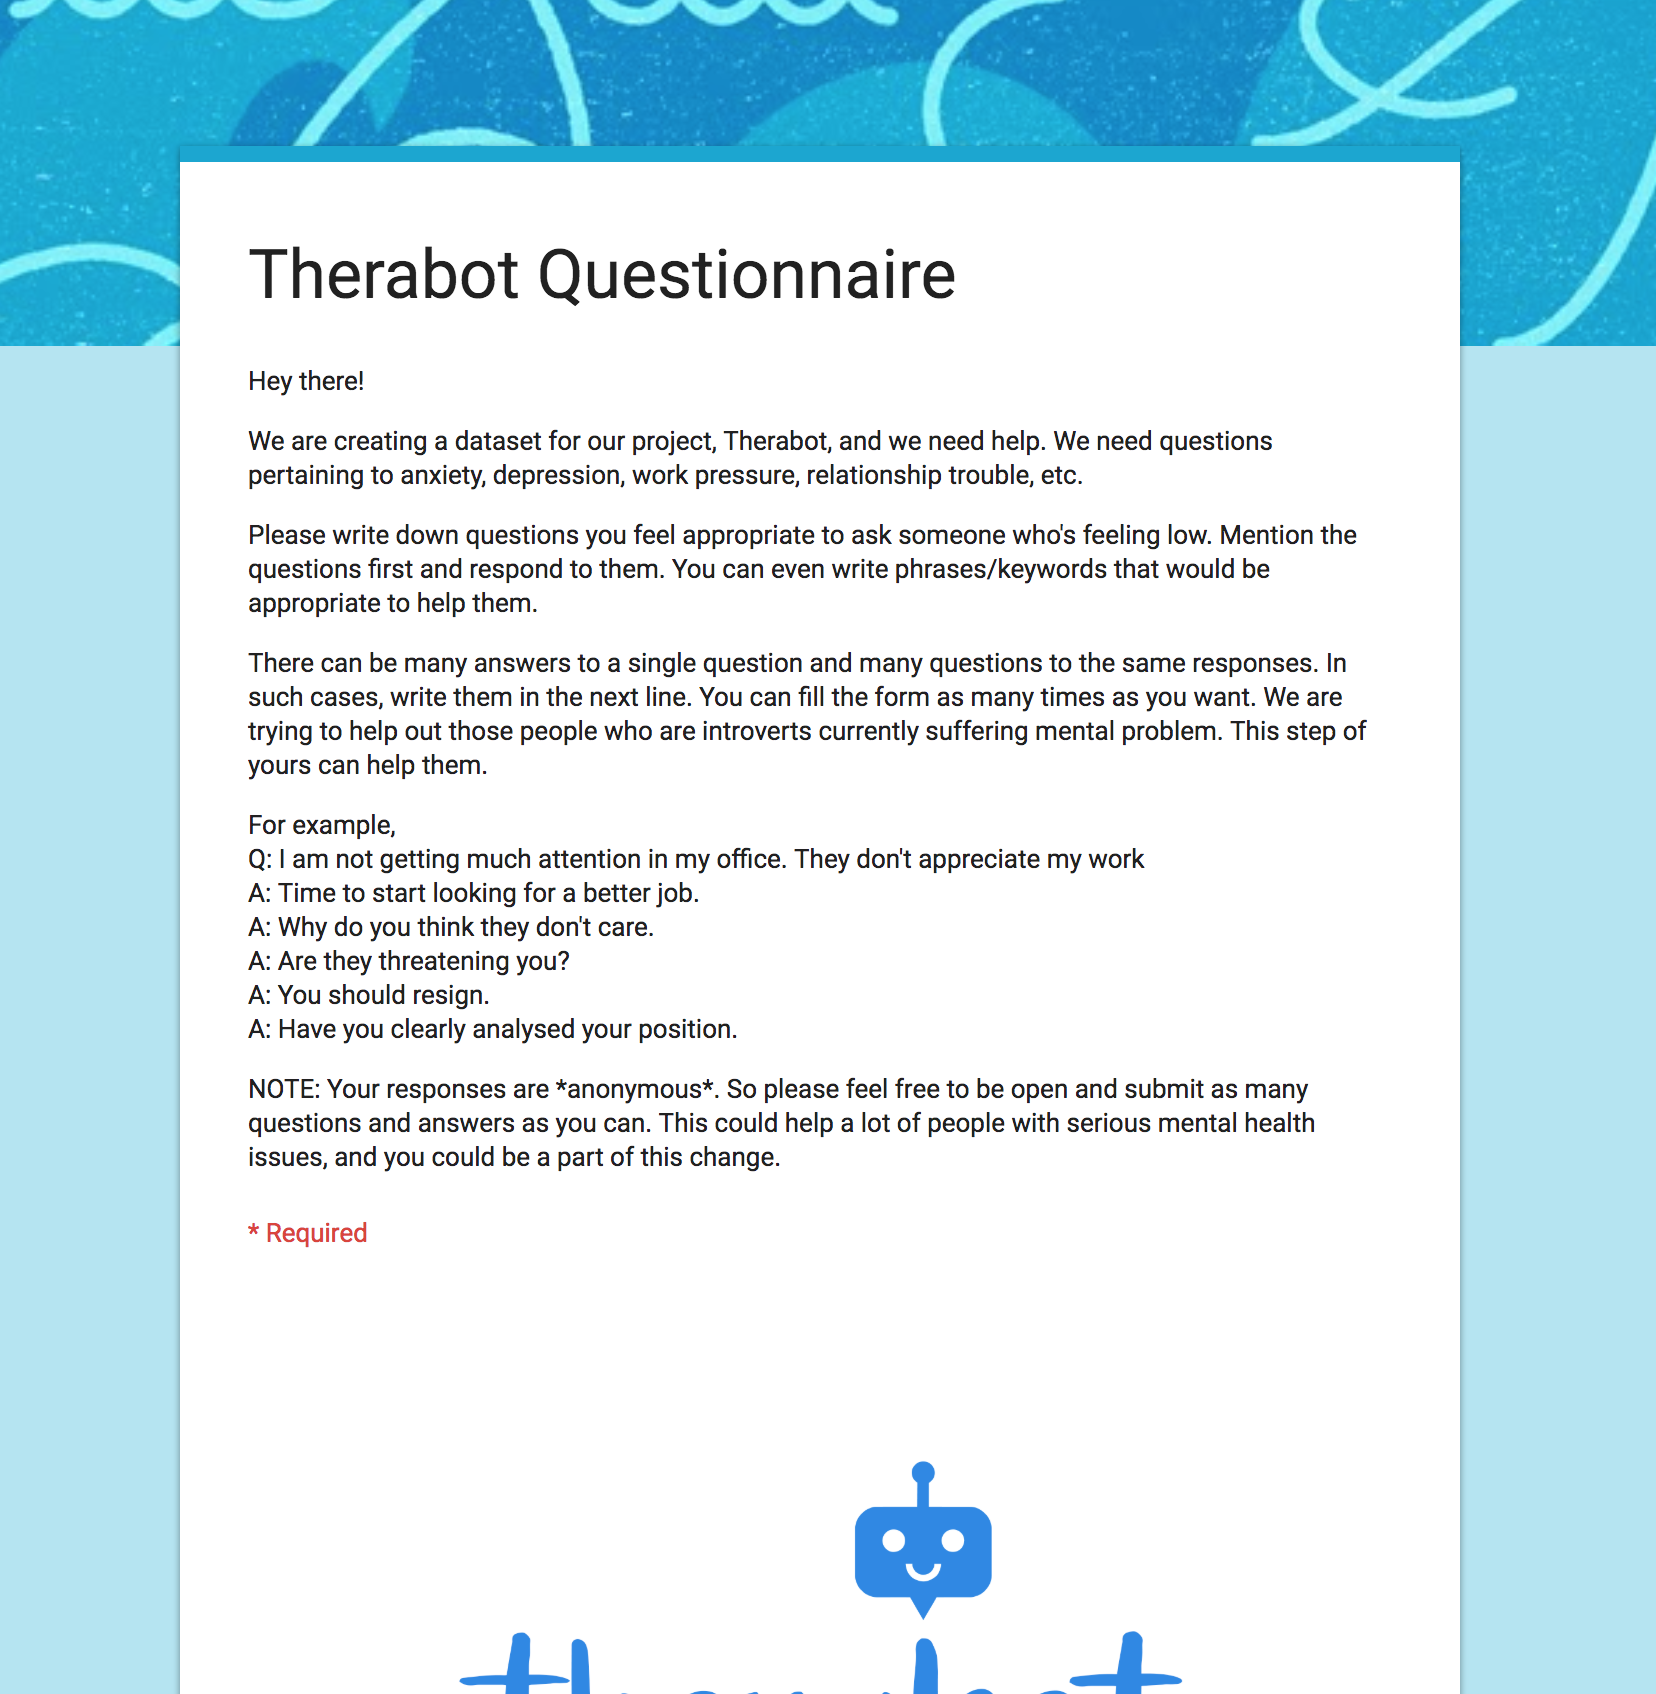
\includegraphics[width=13cm]{images/therabot-questionnaire.png}
    \caption{Therabot Questionnaire}
\end{figure}

We’ve also referred the Facebook Data Corpus and Cornell Movie Corpus for understanding the structure of data and scraped various datasets on Kaggle cherrypicking the from various conversational models to statistical data.

\pagebreak

\subsection{Setting up the Environment}

We’ll need to download the Natural Language Processing Library as well as Tensorflow for higher order numerical computation.

\textbf{Installing NLTK:}
For Windows, Linux and Mac users we recommend installing Anaconda over which the NLP library can be set up. The following command will automatically fetch all the resources and install the Natural Language Toolkit.


\texttt{sudo pip install -U nltk}

\textbf{Installing TensorFlow:}
An environment must be created in in which TensorFlow will be installed. All the necessary pre-requisites and a step-by-step guide to a successful installation are available at https://www.tensorflow.org/install/.

\pagebreak

\subsection{Data Preprocessing}

The accumulated dataset is subjected to a lot of functions which optimize its use during training. This cleaning process is what constitutes the preprocessing.

\subsubsection{Tokenizing}
The dataset contains paragraphs of sentences and well as individual sentences. In some cases, it is necessary to retrieve the sentence as a whole and sometimes as individual words. To facilitate this, the NLTK library has two predefined functions: \texttt{sent\_tokenize} and \texttt{word\_tokenize}.

\begin{figure}[H]
    \centering
    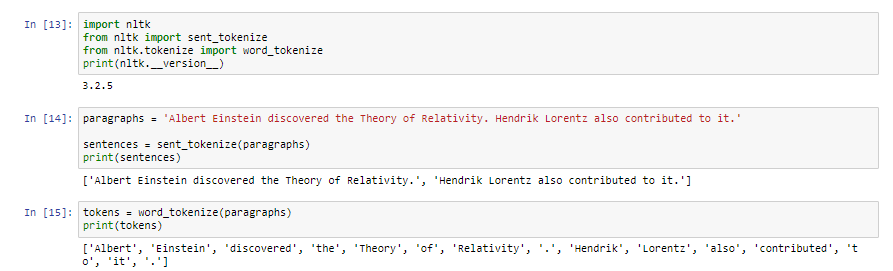
\includegraphics[width=\linewidth]{images/jupyter-notebook-tokenizing.png}
    \caption{Jupyter Notebook - Tokenizing}
\end{figure}

Similarly, punctuation and stop words can also be filtered out.

\subsubsection{Stemming}
While storing the user’s data into Firebase, we need to peddle down the words in these sentences to their purest form or root. This process is called stemming.

\begin{figure}[H]
    \centering
    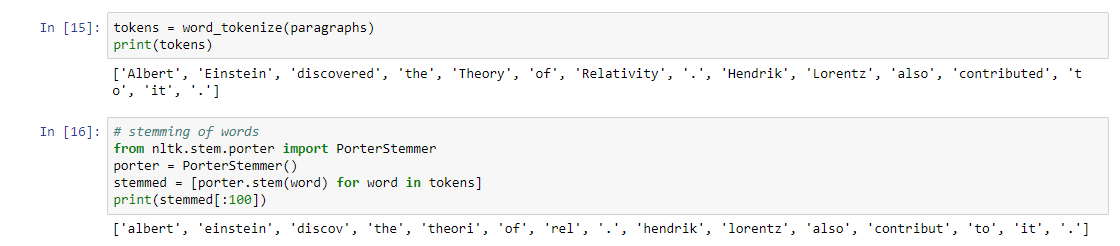
\includegraphics[width=\linewidth]{images/jupyter-notebook-stemming.png}
    \caption{Jupyter Notebook - Stemming}
\end{figure}

\pagebreak

\section{Algorithms}

\subsection{Linear Regression}

When we have a single in put attribute $(x)$ and we want to use linear regression, this is called \textbf{Simple Linear Regression}.

With simple linear regression we want to model our data as follows:
\[
    y = B_{0} + B_{1} * x
\]

This is a line where $y$ is the output variable we want to predict, $x$ is the input variable we know and $B_{0}$ and $B_{1}$ are coefficients we need to estimate.

$B_{0}$ is called the intercept because it determines where the line intercepts the $y$ axis. In machine learning we can call this the bias, because it is added to offset all predictions that we make. The $B_{1}$ term is called the slope because it defines the slope of the line or how $x$ translates into a $y$ value before we add our bias.

The model is called Simple Linear Regression because there is only one input variable $(x)$. If there were more input variables (e.g. $x_{1}, x_{2}$, etc.) then this would be called Multiple Regression.

\pagebreak

\subsection{Gradient Descent}

\textbf{Optimization} refers to the task of minimizing/maximizing an objective function $f(x)$ parameterized by $x$. In machine/deep learning terminology, it’s the task of minimizing the cost/loss function $J(w)$ parameterized by the model’s parameters $w$ \epsilon $R^d$.

Optimization algorithms (in case of minimization) have one of the following goals:
\begin{itemize}
    \item Find the global minimum of the objective function. This is feasible if the objective function is convex, i.e. any local minimum is a global minimum.
    \item Find the lowest possible value of the objective function within its neighborhood. That’s usually the case if the objective function is not convex as the case in most deep learning problems.
\end{itemize}

\textbf{Gradient Descent} is the most common optimization algorithm in machine learning and deep learning. It is a first-order optimization algorithm. This means it only takes into account the first derivative when performing the updates on the parameters. On each iteration, we update the parameters in the opposite direction of the gradient of the objective function $J(w)$ w.r.t the parameters where the gradient gives the direction of the steepest ascent. The size of the step we take on each iteration to reach the local minimum is determined by the learning rate $α$. Therefore, we follow the direction of the slope downhill until we reach a local minimum.

\begin{figure}[H]
    \centering
    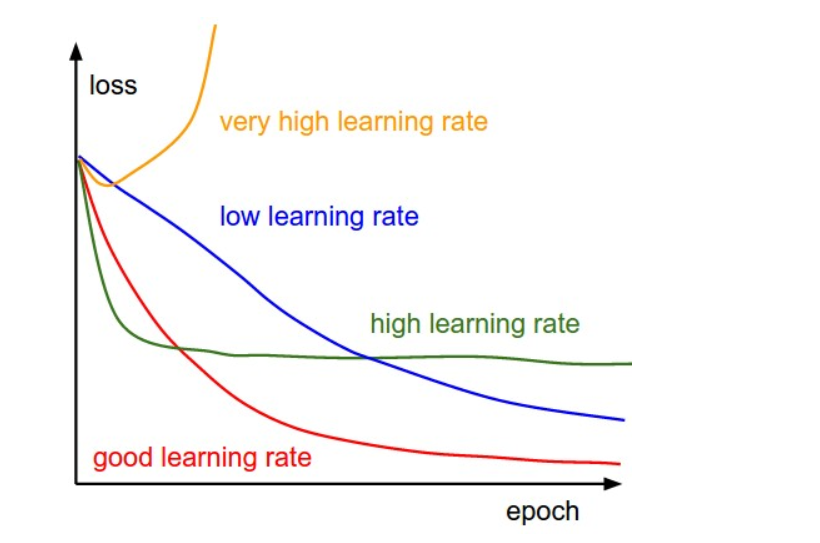
\includegraphics[width=10cm]{images/gradient-descent-different-learning-rates.png}
    \caption{Gradient Descent with Different Learning Rates}
\end{figure}

\pagebreak

\[
    \frac{\delta}{\delta m} = \frac{2}{N} \sum_{i=1}^{N} - x_{i}(y_{i} - (mx_{i} +b))
\]

The coefficients used in simple linear regression can be found using stochastic gradient descent. Linear regression is a linear system and the coefficients can be calculated analytically using linear algebra. Stochastic gradient descent is not used to calculate the coefficients for linear regression in practice (in most cases). Linear regression does provide a useful exercise for learning stochastic gradient descent which is an important algorithm used for minimizing cost functions by machine learning algorithms.

\begin{center}
\begin{tabular}{|c|c|}
    \hline
    $B_{0}$ & $B_{1}$ \\ [0.5ex]
    \hline
    0.01 & 0.01 \\
    \hline
    0.0397 & 0.0694 \\
    \hline
    0.066527 & 0.176708 \\
    \hline
    0.08056049 & 0.21880847 \\
    \hline
    0.1188144616 & 0.410078328 \\
    \hline
    0.1235255337 & 0.4147894001 \\
    \hline
    0.1439944904 & 0.4557273134 \\
    \hline
    0.1543254529 & 0.4970511637 \\
    \hline
    0.1578706635 & 0.5076867953 \\
    \hline
    0.1809076171 & 0.6228715633 \\
    \hline
\end{tabular}
\end{center}

About 10 iterations or 2 epochs is a nice round number and a good place to stop. You could keep going if you wanted. Your values should match closely, but may have minor differences. You can plug each pair of coefficients back into the simple linear regression equation. This is useful because we can calculate a prediction for each training instance and in turn calculate the error.

\pagebreak

\subsection{Logistic Regression}

Logistic Regression is a classification algorithm. It is used to predict a binary outcome (1 / 0, Yes / No, True / False) given a set of independent variables. To represent binary / categorical outcome, we use dummy variables. You can also think of logistic regression as a special case of linear regression when the outcome variable is categorical, where we are using log of odds as dependent variable. In simple words, it predicts the probability of occurrence of an event by fitting data to a logit function.

The fundamental equation of generalized linear model is:
\[
    g(E(y)) = α + βx1 + γx2    
\]

Here, $g()$ is the link function, $E(y)$ is the expectation of target variable and $α + β_{x1} + γ_{x2}$ is the linear predictor ($α, β, γ$ to be predicted). The role of link function is to ‘link’ the expectation of $y$ to linear predictor.

On further deriving the equation, we get this:

\[
    log(\frac{p}{1 - p}) = \beta_{0} + \beta(Age)
\]

This is the equation used in Logistic Regression. Here $(\frac{p}{1-p})$ is the odd ratio. Whenever the log of odd ratio is found to be positive, the probability of success is always more than 50\%. A typical logistic model plot is shown below. You can see probability never goes below 0 and above 1.

\begin{figure}[H]
    \centering
    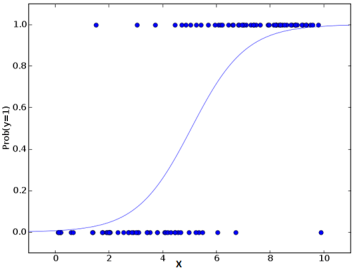
\includegraphics[width=6cm]{images/logistic-regression-plot.png}
    \caption{Typical Logistic Regression Model Plot}
\end{figure}

\pagebreak

\subsection{Softmax Function}

Softmax function calculates the probabilities distribution of the event over ‘$n$’ different events. In general way of saying, this function will calculate the probabilities of each target class over all possible target classes. Later the calculated probabilities will be helpful for determining the target class for the given inputs.

\begin{figure}[H]
    \centering
    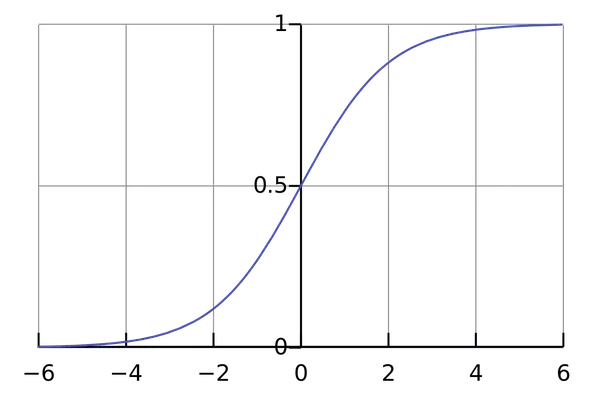
\includegraphics[width=6cm]{images/softmax-function.png}
    \caption{Softmax Function}
\end{figure}

The main advantage of using Softmax is the output probabilities range. The range will 0 to 1, and the sum of all the probabilities will be equal to one. If the softmax function used for multi-classification model it returns the probabilities of each class and the target class will have the high probability.

The formula computes the exponential ($e$-power) of the given input value and the sum of exponential values of all the values in the inputs. Then the ratio of the exponential of the input value and the sum of exponential values is the output of the softmax function.

\[
    P(y = j | z^{(i)}) = \phi_{softmax} (z^{(i)}) = \frac{e^z}{\sum_{j=1}^{k} e^z_k}
\]

\[
    z = w_0x_0 + w_1x_1 + ... + w_mx_m = \sum_{i=0}^{m} w_ix_i = w^Tx
\]

The softmax function is often used in the final layer of a neural network-based classifier. Such networks are commonly trained under a log loss (or cross-entropy) regime, giving a non-linear variant of multinomial logistic regression.

\pagebreak

\section{Diagrams}

\subsection{Data Flow Diagram}

A Data Flow Diagram (DFD) is traditional visual representation of the information flows within a system. A neat and clear DFD can depict a good amount of the system requirements graphically. It can be manual, automated, or combination of both. It shows how information enters and leaves the system, what changes the information and where information is stored. The purpose of a DFD is to show the scope and boundaries of a system as a whole.

There are four major components or external agents involved in the system:
\begin{itemize}
    \item User
    \item DialogFlow Framework
    \item Machine Learning Model
    \item Firebase Database
\end{itemize}

\begin{figure}[H]
    \centering
    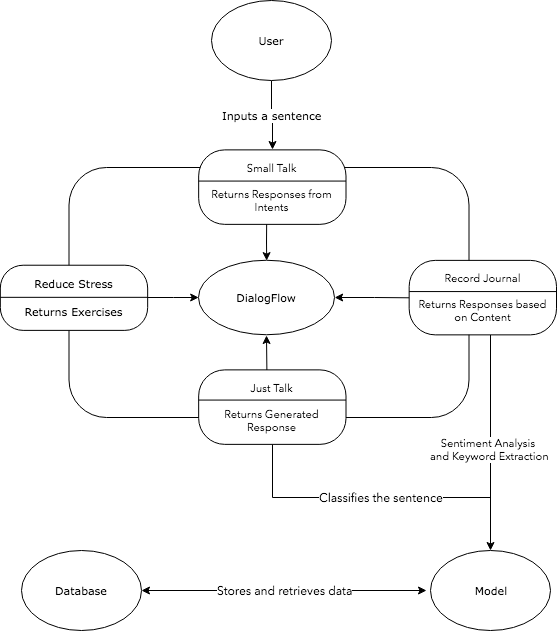
\includegraphics[width=10cm]{images/data-flow-diagram.png}
    \caption{Data Flow Diagram}
\end{figure}

\pagebreak

\subsection{Sequence Diagram}

A sequence diagram shows object interactions arranged in time sequence. It depicts the objects and classes involved in the scenario and the sequence of messages exchanged between the objects needed to carry out the functionality of the scenario.

We have two different sequence diagrams here:
\begin{itemize}
    \item Onboarding Phase
    \item Regular Conversations
\end{itemize}

\begin{figure}[H]
    \centering
    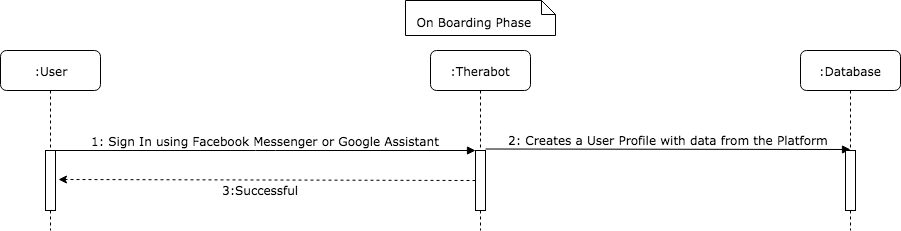
\includegraphics[width=\linewidth]{images/sequence-diagram-onboarding-phase.png}
    \caption{Sequence Diagram - Onboarding Phase}
\end{figure}

\begin{figure}[H]
    \centering
    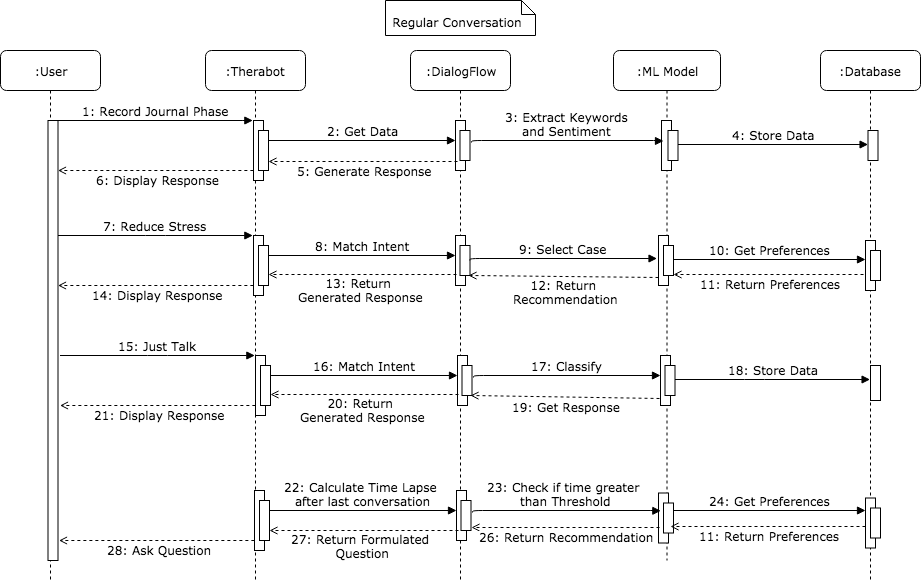
\includegraphics[width=\linewidth]{images/sequence-diagram-regular-conversations.png}
    \caption{Sequence Diagram - Regular Conversations}
\end{figure}